\documentclass{article}
\usepackage[T1]{fontenc}
\usepackage[utf8]{inputenc}
\usepackage[portuguese]{babel}

\title{Lista 4 \\
\large Equações Diferenciais Parciais}
\author{Lucas Emanuel Resck Domingues}
\date{Outubro de 2020}

\usepackage{natbib}
\usepackage{graphicx}
\usepackage{amsmath}
\usepackage{hyperref}
\usepackage{listings}
\usepackage{amssymb}
\usepackage{cases}

%Hyperlinks
\usepackage{hyperref}
\hypersetup{
    colorlinks=true,
    allcolors=,  % Nothing change colors
    urlcolor=blue  % URL changes color
}

\begin{document}

    \maketitle
    
    \section*{Exercícios teóricos}

        \begin{enumerate}
            \item            
                \begin{enumerate}
                    \item Essa função é especial: ela é seno.
                        Sendo assim, podemos escolher os coeficientes
                        $a_n$ e $b_n$ tais que encontremos o seno de $5x$.
                        Da expressão da série de Fourier, basta que escolhamos
                        todos os coeficientes iguais a zero, com exceção de $b_5 = 1$.
                        Então:
                        
                        \begin{align*}
                            a(x) &= \dfrac{a_0}{2} + \sum_{m=1}^{\infty} \left(a_m \cos \left(\dfrac{m \pi x}{L}\right) + b_m \sin \left(\dfrac{m \pi x}{L}\right)\right) \\
                            &= \sin \left(\dfrac{5 \pi x}{L}\right) \\
                            &= \sin(5x)
                        \end{align*}

                    \item Calculemos os coeficientes:
                    
                        $$a_0 = \dfrac{1}{\pi} \int_{-\pi}^{\pi} \sin(5x + \alpha) dx = 0$$

                        Se $n \ne 0$:
                        
                        \begin{align*}
                            a_n &= \dfrac{1}{\pi} \int_{-\pi}^{\pi} \sin(5x + \alpha) \cos(nx) dx \\
                            &= \begin{cases}
                                -\dfrac{2n\sin(\alpha)\sin(\pi n)}{\pi(n^2-25)}, & n \ne 5\\
                                \sin(\alpha), & n = 5
                            \end{cases} \\
                            &= \begin{cases}
                                0, & n \ne 5\\
                                \sin(\alpha), & n = 5
                            \end{cases}
                        \end{align*}

                        Agora para $b_n$:

                        \begin{align*}
                            b_n &= \dfrac{1}{\pi} \int_{-\pi}^{\pi} \sin(5x + \alpha) \sin(nx) dx \\
                            &= \begin{cases}
                                -\dfrac{10\cos(\alpha)\sin(\pi n)}{\pi(n^2-25)}, & n \ne 5\\
                                \cos(\alpha), & n = 5
                            \end{cases} \\
                            &= \begin{cases}
                                0, & n \ne 5\\
                                \cos(\alpha), & n = 5
                            \end{cases}
                        \end{align*}

                        Então:
                        
                        \begin{align*}
                            b(x) &= \dfrac{a_0}{2} + \sum_{m=1}^{\infty} \left(a_m \cos \left(\dfrac{m \pi x}{L}\right) + b_m \sin \left(\dfrac{m \pi x}{L}\right)\right) \\
                            &= a_5 \cos(5x) + b_5 \sin(5x) \\
                            &= \sin(\alpha) \cos(5x) + \cos(\alpha) \sin(5x)
                        \end{align*}

                    \item
                        $$a_0 = \dfrac{1}{\pi} \int_{-\pi}^{\pi}c(x)dx = \dfrac{1}{\pi} \int_{0}^{\pi} 1 dx = 1$$

                        $$a_n = \dfrac{1}{\pi} \int_{0}^{\pi} \cos(nx) dx = 0$$

                        $$b_n = \dfrac{1}{\pi} \int_{0}^{\pi} \sin(nx) dx
                        = \dfrac{-\cos(n\pi)+1}{n\pi} = \begin{cases}
                            0, &n \text{ par} \\
                            \dfrac{2}{n\pi}, &n \text{ ímpar}
                        \end{cases}$$

                        $$c(x) = \dfrac{1}{2} + \sum_{n=1}^\infty \dfrac{2\sin(nx)}{n\pi}
                        = \dfrac{1}{2} + \dfrac{2}{\pi}\sum_{m=1}^\infty \dfrac{\sin((2m+1)x)}{(2m+1)}$$

                    \item
                        $$a_0 = \int_{-1}^{1}x dx = 0$$
                        
                        $$a_n = \int_{-1}^{1} x\cos(n\pi x) dx = 0$$
                        afinal o integrando é uma função ímpar.

                        $$b_n = \int_{-1}^{1} x \sin(n\pi x) dx = \dfrac{2 \sin(\pi n) - 2 \pi n \cos(\pi n)}{\pi^2n^2}$$

                        $$c(x) = \dfrac{2}{\pi^2} \sum_{n=1}^{\infty} \dfrac{\sin(\pi n) - \pi n \cos(\pi n)}{n^2} \sin(n\pi x)$$
                \end{enumerate}

            \item Veremos que a equação de diferenças parcial pode ser formulada
                como uma equação diferencial matricial. Vamos resolvê-la e verificar 
                que a base de Fourier nos ajuda a encontrar os coeficientes da solução
                da equação diferencial matricial.

                Temos um polígono com $n$ lados e $n$ vértices
                Sejam os vértices $x_1, \cdots, x_n$.
                Veja que a matriz de adjacência é dada:

                $$A = \begin{bmatrix}
                    0 & 1 & 0 & 0 & \cdots & 0 & 1 \\
                    1 & 0 & 1 & 0 &\cdots & 0 & 0 \\
                    0 & 1 & 0 & 1 &\cdots & 0 & 0 \\
                    \vdots & \vdots & \vdots & \vdots & \ddots & \vdots & \vdots \\
                    1 & 0 & 0 & 0 & \cdots & 1 & 0 \\
                \end{bmatrix}$$

                Então a matriz do laplaciano $L$ é dada por

                $$L = D - A = \begin{bmatrix}
                    2 & -1 & 0 & 0 & \cdots & 0 & -1 \\
                    -1 & 2 & -1 & 0 &\cdots & 0 & 0 \\
                    0 & -1 & 2 & -1 &\cdots & 0 & 0 \\
                    \vdots & \vdots & \vdots & \vdots & \ddots & \vdots & \vdots \\
                    -1 & 0 & 0 & 0 & \cdots & -1 & 2 \\
                \end{bmatrix}$$

                sendo $D$ a matriz diagonal com os graus de cada vértice.

                Nosso polígono regular tem $n$ lados. Considere o vetor $$w(t) = (u(x_1, t), u(x_2, t), \cdots, u(x_n, t))$$

                Ele descreve a temperatura em todos os vértices do polígono no tempo $t$.
                Porém, sabemos que

                $$w'(t) = -L w(t)$$

                (a simples multiplicação de $-L$ por $w$ resulta na equação de diferenças parcial do enunciado,
                porém para todos os valores de $x$ de uma vez só).
                Sendo assim, temos uma equação diferencial matricial.
                Observe que $L$ é uma matriz de convolução.
                
                Vamos considerar agora a base de Fourier $\{f_1, \cdots, f_n\}$, sendo

                $$f_i = \dfrac{1}{\sqrt{n}} \left((w^i)^0, (w^i)^1, \cdots, (w^i)^{n-1}\right)$$

                Nós sabemos que a base de Fourier é um conjunto ortonormal de cardinalidade $n$, então é uma base para o espaço
                $\mathbb{C}^n$. Ora, então existem $c_1(t), \cdots, c_n(t)$ tais que

                $$w(t) = \sum_{i=1}^n c_i(t)f_i$$

                Segue que

                $$w'(t) = \sum_{i=1}^n c_i'(t)f_i$$

                Porém, também sabemos que a base de Fourier diagonaliza matrizes de convolução. Portanto:

                $$\sum_{i=1}^n \dfrac{\mathrm{d}c_i}{\mathrm{d}t}(t)f_i = -L\sum_{i=1}^nc_i(t)f_i = -\sum_{i-1}^n c_i(t)\lambda_if_i$$

                sendo $\lambda_i$ autovalor associado ao autovetor $f_i$.
                O fato dos autovetores serem ortonormais nos leva a

                $$\dfrac{\mathrm{d}c_i}{\mathrm{d}t}(t) = -c_i(t)\lambda_i$$

                cuja solução conhecemos:

                $$c_i(t) = c_i(0) e^{-\lambda_i t}$$

                Para obtermos $c_i(0)$, fazemos

                $$\left<u(., 0), f_i\right> = \left<w(0), f_i\right> = \left<\sum_{i=1}^n c_i(0)f_i, f_i\right> = c_i(0)$$

                Para obtermos $\lambda_i$, já sabemos que basta $\lambda_i = \left<h, f_i\right>$,
                sendo $h$ o vetor que gera a matriz de convolução. Por exemplo, no nosso caso,

                $$h = (2, -1, 0, 0, \cdots, 0, -1)$$

                Resumindo: obtemos $\lambda_i$, $c_i(0)$, $c_i(t)$ e, finalmente, $w(t)$.

            \item 
            % Temos a EDP
            %     $$\begin{cases}
            %         u_t + c u_x = 0 \\
            %         u(x, 0) = f(x)
            %     \end{cases}$$
            %     sendo $f$ periódica com período $2\pi$

            \item Vamos resolver a seguinte EDP pelo método de
                separação de variáveis:

                \begin{numcases}{f(x)=}
                    u_{tt} = u_{xx}, & $(x, t) \in (0, L)\times\mathbb{R}_+^*$ \label{eq:1} \\
                    u(x, 0) = \sin(5x), & $x \in (0, L)$ \label{eq:2} \\
                    u_t(x, 0) = 0, & $x \in (0, L)$ \label{eq:3}
                \end{numcases}

                Iniciamos supondo $u(x, t) = X(x) T(t)$.
                Observe a equação \ref{eq:2}. Dela, concluímos que

                $$X(x)T(0) = \sin(5x) \Rightarrow X(x) = \dfrac{\sin(5x)}{T(0)}$$

                Observe que não vale que $T(0) = 0$, pois senão $\sin(5x) = 0$ sempre.
                Por isso vale a divisão.

                Pela equação \ref{eq:1}:

                \begin{align*}
                    u_{tt} = u_{xx} &\Rightarrow X(x)T''(t) = X''(x)T(t) \\
                    &\Rightarrow \dfrac{T''(t)}{T(t)} = \dfrac{X''(x)}{X(x)}
                \end{align*}

                Fixe $x$, varie $t$. Então $\dfrac{T''(t)}{T(t)}$ é constante.
                Análogo para $X$. Chamemos essa constante de $\lambda$.
                Pelo fato de que $X''(x) = \lambda X(t)$, além de que sabemos a expressão de $X(t)$,
                temos que $\lambda = -25$.

                Vamos desenvolver agora $T''(t) = \lambda T(t) = -25 T(t)$.
                Estamos resolvendo uma EDO de 2ª ordem homogênea. Busquemos as raízes de

                $$y^2+25 = 0$$

                Então as raízes são $\pm 5i$, de modo que a solução geral dessa EDO é

                \begin{align*}
                    T(t) &= e^{0t} (A \cos(5t) + B\sin(5t)) \\
                    &= A \cos(5t) + B\sin(5t)
                \end{align*}

                Vamos utilizar a equação \ref{eq:3} para nos ajudar a determinar o coeficiente $B$.
                
                \begin{align*}
                    u_t(x, 0) = 0 &\Rightarrow X(x) T'(0) = 0 \\
                    &\Rightarrow T'(0) = 0
                \end{align*}

                Ora, se não fosse isso, então $X(x) = 0$, o que não faz sentido.

                \begin{align*}
                    T'(0) = 0 &\Rightarrow -5A \sin(0) + 5B\cos(0) = 0 \\
                    &\Rightarrow B = 0 \\
                    &\Rightarrow T(t) = A \cos(5t)
                \end{align*}

                Concluímos, portanto, que

                $$u(x, t) = X(x)T(t) = \dfrac{\sin(5x)}{A \cos(0)}A \cos(5t) = \cos(5x)\sin(5x)$$

                Observe que essa função satisfaz a todas as condições iniciais.
        \end{enumerate}

    \section*{Exercícios computacionais}

        \begin{enumerate}
            \item O programa para o Afinador de Fourier
                foi escrito em \textit{Matlab} e pode ser conferido
                no Apêndice \ref{appendix:tuner}.

                O programa toma como entrada o diretório do arquivo,
                lê o arquivo, calcula a transformada de Fourier do vetor, extrai
                a frequência com maior amplitude e calcula a frequência real
                com maior amplitude.

                Para o áudio \textit{CordaViolao2.wav}, o programa detectou
                predominância da frequência 331 Hz, que representa uma nota E,
                provavelmente a corda 1 do violão.

            \item \begin{enumerate}
                    \item O gráfico dos pontos $(x_i, y_i)$ pode ser observado na Figura \ref{fig:octopus}.
                    
                        \begin{figure}[!h]
                            \centering
                            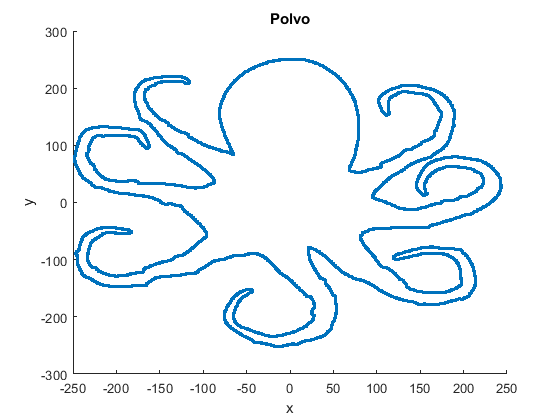
\includegraphics[width=\textwidth]{octopus.png}
                            \caption{Pontos $(x_i, y_i)$.}
                            \label{fig:octopus}
                        \end{figure}

                    \item Seja $x_0 = (x_1, \cdots, x_n)$.
                        Usando da analogia de que esse vetor representa as temperaturas iniciais
                        nos vértices de um grafo circular com $n$ vértices,
                        vamos utilizar a equação do calor para calcular as temperaturas
                        para diferentes instantes de tempo, na esperança que as diferenças
                        de temperatura sejam suavizadas, ou seja, o gráfico dos pontos seja suavizado.

                        Vamos utilizar a solução para a equação do calor,
                        $x(t) = e^{-c t L} x_0$, para calcular as temperaturas
                        e suavizar o gráfico. Segue:

                        \begin{align*}
                            x(t) &= e^{-c t L} x_0 \\
                            &= F e^{D} F^{-1} x_0 \\
                            &= F e^{D} \textrm{fft}(x_0) \\
                        \end{align*}

                        sendo $\textrm{fft}$ a transformada discreta de Fourier,
                        $F$ a matriz com as colunas sendo a base de Fourier.
                        $D$ é uma matriz diagonal com os autovalores de
                        $-ctL$.

                        É conhecido que os autovalores de $-ctL$ são $\textrm{fft}(-cth)$,
                        sendo $h$ a primeira linha de $L$. Então segue que:

                        Considere que $x_{0,F}$ representa $x_0$ na base de Fourier.
                        Veja que $e^D \cdot x_{0, F}$ é fácil de ser calculado:
                        basta realizar a multiplicação elemento a elemento de
                        $$\exp(\lambda) = \exp((\lambda_1, \cdots, \lambda_n)) = \left(e^{\lambda_1}, \cdots, e^{\lambda_n}\right)$$
                        ou seja, o vetor com a exponencial de cada autovalor de $-ctL$, e
                        $$x_{0, F}$$
                        nosso vetor $x_0$ na base de Fourier. É o que será feito.

                        Sendo assim, ao final, basta aplicar $\textrm{ifft}$ para voltarmos
                        à base canônica:

                        \begin{align*}
                            x(t) &= F e^{D} \textrm{fft}(x_0) \\
                            &= \textrm{ifft}\left(e^{D} \textrm{fft}(x_0)\right) \\
                        \end{align*}

                        Foi implementada uma função em \textit{Matlab} que faz isso e
                        também constrói o gráfico.

                \end{enumerate}
        \end{enumerate}

    \newpage

    \appendix

        \section{Afinador de Fourier}
            \label{appendix:tuner}

            \begin{lstlisting}[language=Matlab]
function freq = fourier_tuner(filepath)
    [y, Fs] = audioread(filepath);
    yhat = fft(y);
    % This is because of symmetry of Fourier coefficients
    max_freq = ceil(length(yhat)/2);
    [~, cicles] = max(abs(yhat(1:max_freq)));
    freq = cicles/(length(y)/Fs);
end
            \end{lstlisting}

\end{document}